\chapter{Einleitung} \label{chap:Einleitung}
\thispagestyle{empty}
Gestzlichen Bestimmung zur Erhöhung der Sicherheit von sowohl den Insassen eines Fahrzeugs als auch anderer Verkehrsteilnehmer hat zu einer signifikanten Senkung der Mortalitätsrat bei Verkehrsunfällen beigetragen und den Straßenverkehr in den letzten Jahren wesentlich sicherer gemacht, siehe Abbildung \ref{fig:Statistik_Tote}.
\begin{figure} [H]
    \centering
    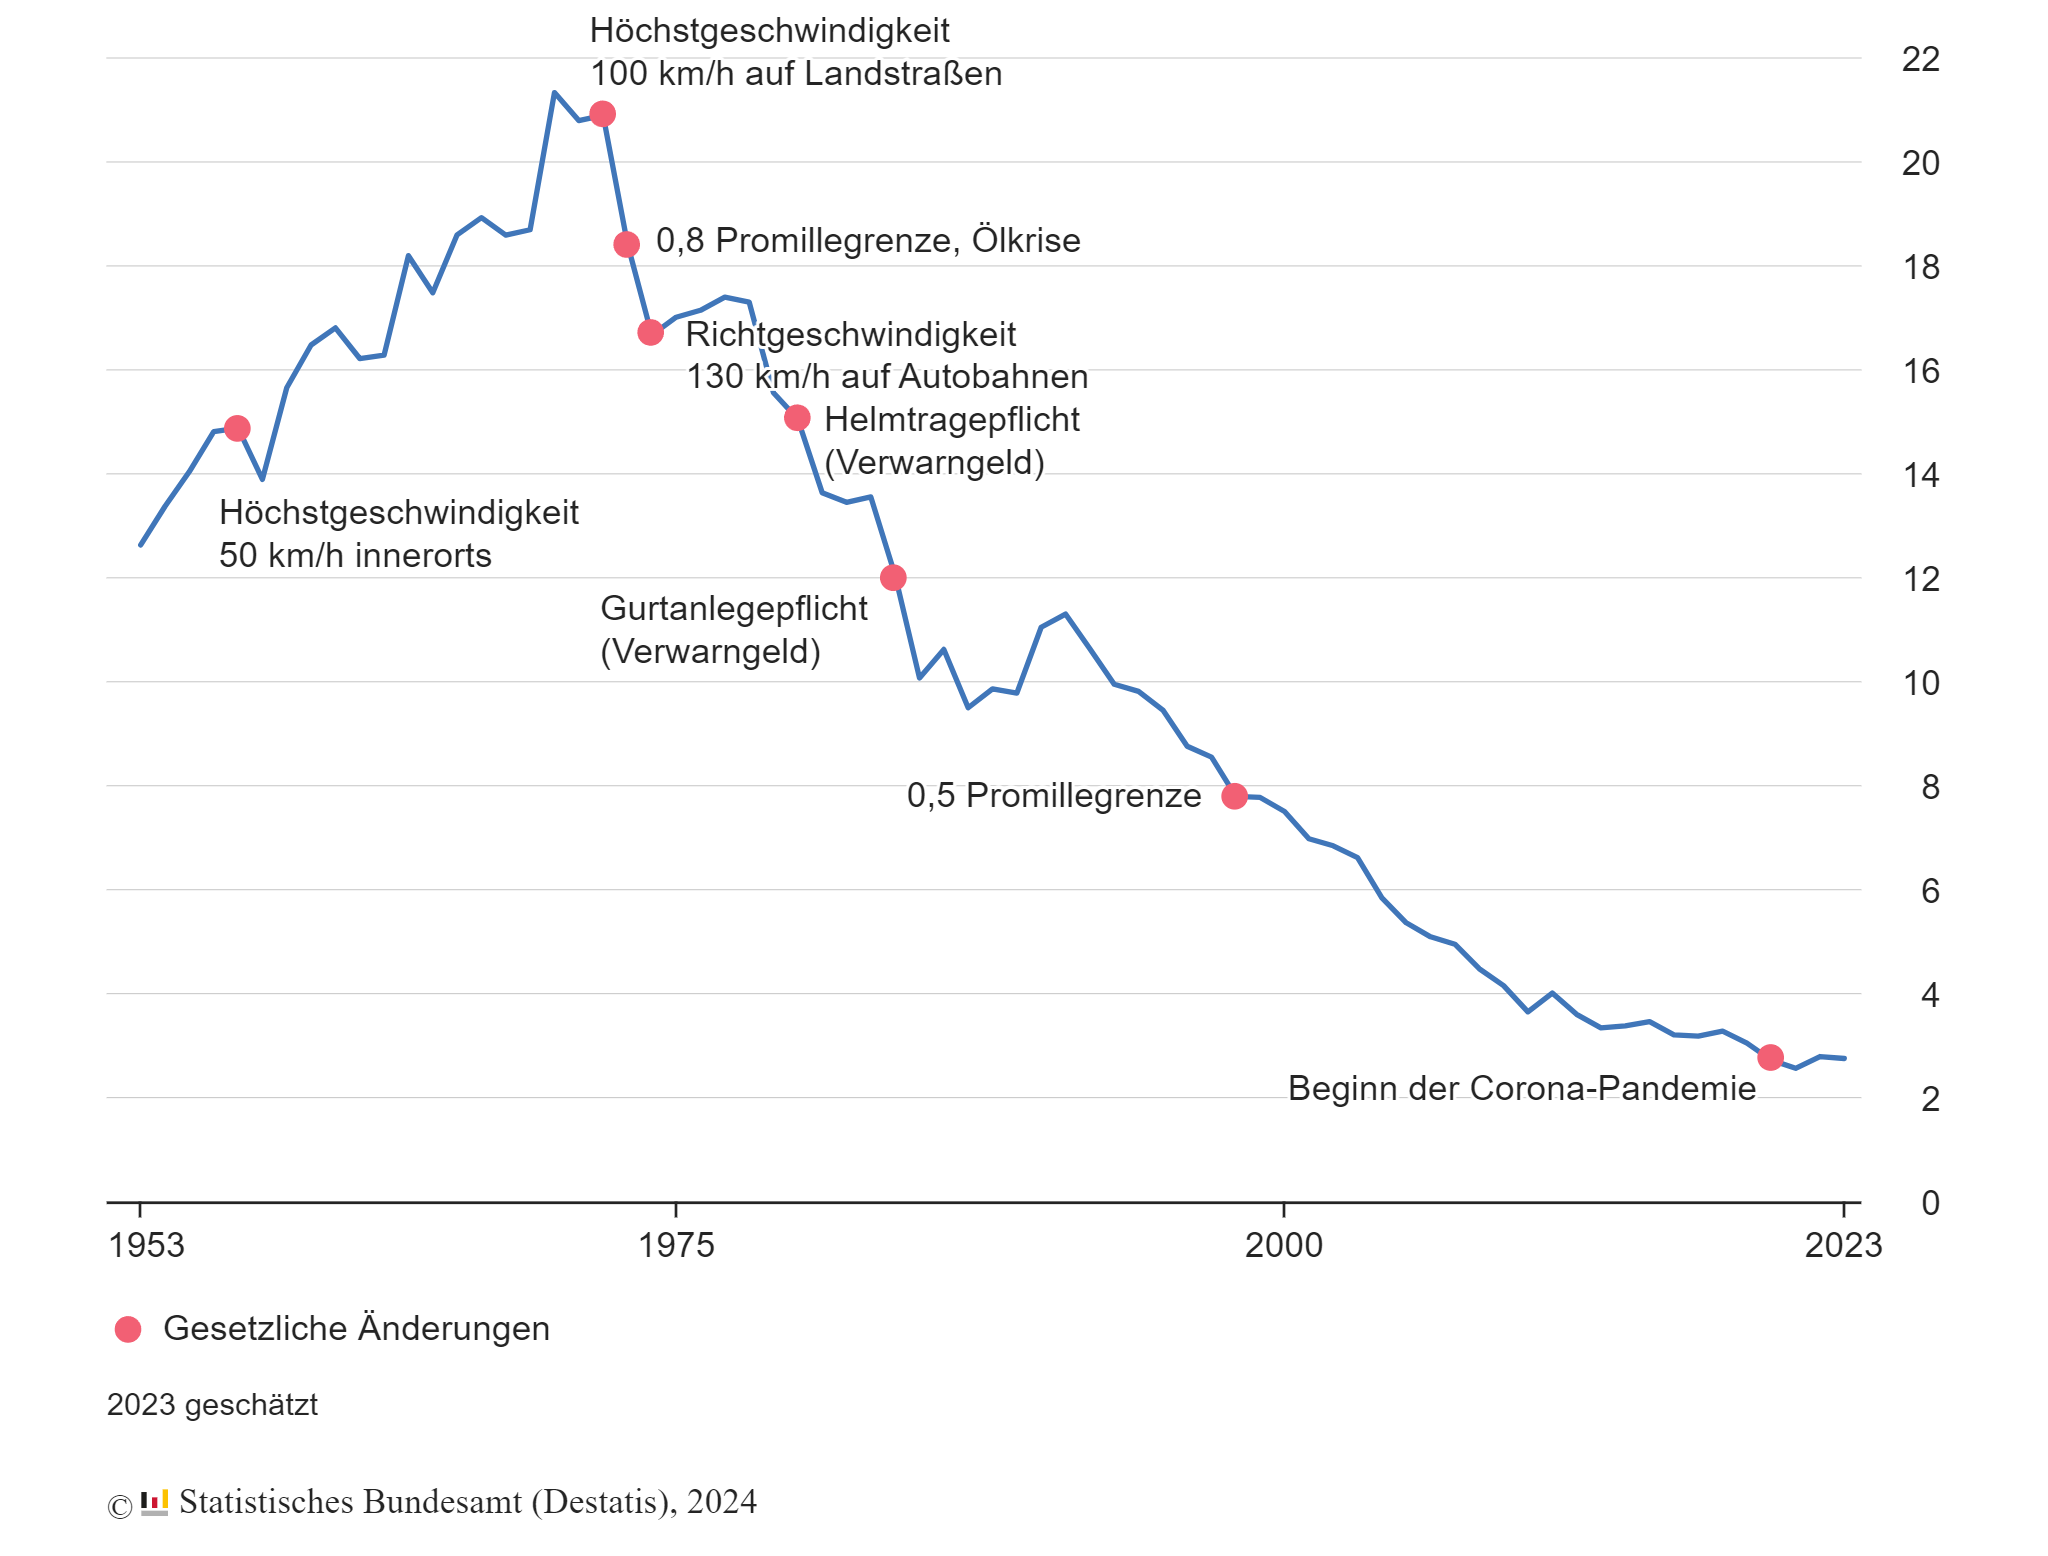
\includegraphics[width=0.9\textwidth]{figures/1_Einleitung/verkehrsunfaelle-getoetete-jahr.png}
    \caption{Bei Verkehrsunfällen Getötete pro Jahr in Tausend \cite{StBA2021}}
    \label{fig:Statistik_Tote}
\end{figure}
\noindent Im Jahr 2021 gab es über 250.000 Unfälle mit Personenschaden auf deutschen Straßen. In 88\% der Fälle ist die Ursache auf ein Fehlverhalten der Fahrzeugführer zurückzuführen \cite{StBA2021}. Der Einsatz von automatisierten Fahrzeugen kann zu einem weiteren "Knick" in den Statistiken führen, indem es den Fahrer durch Einsatz von intelligenten Asstenzsystemen unterstützt oder die menschliche Fehlerkomponente gänzlich beseitigt, indem ein Fahrzeug vollständig autonom fährt.

Um die Sicherheit der Fahrzeuge zu gewährleisten muss sowhl das Gesamtsystem als auch alle Teilsysteme intensiv getestet werden. Eines dieser Teilsystem für das hochautomatisierte Fahren ist die Regelung der Längs- und Querführung des Fahrzeugs. Bei der IAV\footnote{\url{https://www.iav.com/}} geschieht dies durch einen modellprädiktiven Pfadfolgeregler.\bigskip

\noindent\textbf{Aufgabenstellung}\smallskip

\noindent Im Rahmen des Praktikums soll eine automatisierte Teststrategie für einen modellprädiktiven Pfadfolgeregler (MPFC) konzeptioniert und implementiert werden.

Modellprädiktive Regler (MPC) eignen sich hervorragend für die Vorhersage und Regelung dynamischer System, weshalb sie in vielen Industriezweigen, einschließlich der Automobilindustrie, Anwendung finden. Im Bereich des hochautomatisierten Fahrens können mithilfe von MPC in Echtzeit Fahrentscheidungen, die sowohl sicherheits- als auch komfortrelevante Anforderungen erfüllen, getroffen werden. Um die Sicherheit und Zuverlässigkeit des Systems sicherzustellen sollen realitätsnahe Fahrszenarien ermittelt und anhand von festgelegten Key Performance Indicators (KPIs) bewertet werden. Dieser Prozess soll automatisiert in einer CI Pipeline ablaufen.\medskip

\noindent Es sind die folgenden Teilaufgaben umzusetzen:
\begin{itemize}
    \item Konzeptentwicklung für das automatisierte, szenariobasierte Testen der MPFC unter Verwendung der bestehenden Simulationsumgebung
    \item Definition und Parametrierung geeigneter Fahrszenarien
    \item Definition von Key Performance Indicators zur Beurteilung der Leistung der Regelung
    \item Einbindung in eine Gitlab CI Pipeline
    \item Dokumentation der Ergebnisse
\end{itemize}
